%!bin/usr/pdflatex
% Thomas J. Leeper
% Aarhus University
% January 29, 2013
% MTurkR Article for The Political Methodologist

\documentclass[11pt]{article}
\usepackage{titlesec}
\usepackage{graphicx,setspace,hyperref,amsmath,amsfonts,times,multirow,ccaption,tabularx,fancyvrb,booktabs,mdwlist,verbatim}
\usepackage[top=1in, bottom=1in, left=1in, right=1in]{geometry}
\setlength{\marginparwidth}{.5in}
\usepackage{natbib}
\bibpunct{(}{)}{;}{a}{}{,} %set in-line reference punctuation
\setlength{\bibsep}{0.1in} %set spacing between references
\setlength{\bibhang}{.5in} %set hanging indent for references
\setlength{\parindent}{0.5in}
\renewcommand\bibsection{\section*{\refname}} %Changes "Bibliography" to "References"
\expandafter\def\expandafter\quote\expandafter{\quote\singlespacing} %single space quote environment
\usepackage[T1]{fontenc}
\usepackage{lmodern}
\hypersetup{
    bookmarks=true,         % show bookmarks bar?
    unicode=false,          % non-Latin characters in Acrobat’s bookmarks
    pdftoolbar=true,        % show Acrobat’s toolbar?
    pdfmenubar=true,        % show Acrobat’s menu?
    pdffitwindow=false,     % window fit to page when opened
    pdfstartview={FitH},    % fits the width of the page to the window
    pdftitle={MTurkR},    % title
    pdfauthor={Thomas J. Leeper},     % author
    pdfsubject={MTurkR},   % subject of the document
    pdfkeywords={Amazon Mechanical Turk} {MTurk} {R} {API} {Crowdsourcing}, % list of keywords
    pdfnewwindow=true,      % links in new window
    pdfborder={0 0 0}
}

\title{Crowdsourcing with R and the MTurk API}
\author{Thomas J. Leeper\thanks{Department of Political Science, Aarhus University}}

\begin{document}

\maketitle

{\abstract This article introduces the collection of social science data through the Amazon Mechanical Turk (MTurk) crowdsourcing platform, taking advantage of a new package for R that connects to the MTurk API. Through two use cases --- (1) human coding of materials and (2) a panel survey-experiment --- the utility of MTurk as a research platform is demonstrated, as is the use of R to leverage cloud-based data APIs.}

\singlespacing

Political scientists are in constant need of human-generated data. Responses to survey questions and reactions to experimental stimuli, manual coding of visual, auditory, and textual data, and the recorded behavior of individuals engaged in naturalistic or artificial behaviors are the bread and butter of contemporary quantitative research on politics. Yet access to large numbers of humans capable of producing these data is often a major logistic and financial challenge for researchers doing everything from large coding projects to pretesting of questionnaires to the recruitment of participants for full research studies. This search for humans willing to generate the kinds of data social scientists demand has led to major recent interest in online data collection generally \citep[e.g.,][]{Iyengar2010, IyengarVavreck2011, VavreckIyengar2011} and, more recently, crowdsourcing platforms in particular \citep{Schmidt2010, ChenMenezesBradley2011} to provide these kinds of data at low cost. Among these platforms, Amazon Mechanical Turk (MTurk) stands out as one of the largest and most useful platforms for political science research \citep{BerinskyHuberLenz2010}.%\footnote{The possibilities offered by MTurk have produced a huge surge in working, conference, and forthcoming papers \citep[for some political science examples, see][]{HirschKangBodenhausen2012, Berinsky2011, Lenz2010, GaskinJerit2012, ArceneeauxJohnson2012, Sheagley2012, Thorson2012, NyhanReifler2011, Arceneaux2012, MunsonResnick2010}. Most of these papers leverage MTurk for experimental research; I am unaware of any that leverage MTurk for large-scale data coding.}

Leveraging MTurk to move traditionally pencil-and-paper processes managed locally (like laboratory experiments or the hand-coding of materials by undergraduate research assistants) into a cloud-based process can dramatically lower the time and resource expenditure involved with such efforts, as well as streamline research workflow. This article advocates for and describes how to move these social science data needs into the cloud using an R package called MTurkR \citep{Leeper2012c}, while also encouraging the development of packages that connect researchers to potentially valuable sources of API-based data. Integrating data APIs into R enables researchers to work with data in a familiar programming environment, directly link data collection and data analysis (thereby eliminating the number of steps and amount of time involved), and aid the reproducibility of research by focusing on using (and making) publicly available data that can be readily accessed from the cloud using code that can be shared to produce identical results.\footnote{Another approach is the \href{http://cran.r-project.org/web/packages/dvn/index.html}{dvn} package, which provides access to The Dataverse Network repository API \citep{Leeper2013} or the \href{http://ropensci.org/}{ROpenSci} project, which does the same for a large number of (mostly natural science) APIs.}

\section{MTurk: Introduction and Core Concepts}
MTurk is a crowdsourcing platform designed to provide ``human intelligence'' for tasks that cannot be readily, affordably, or feasibly automated \citep{Amazon2012}. The service provides researchers with useful infrastructure for the generation of common social science data. While many early adopters of MTurk as a data generation tool came from computer science \citep{MasonSuri2011, KitturChiSuh2008}, more recent attention has emerged among social scientists \citep{BuhrmesterKwangGosling2011, BerinskyHuberLenz2010, PaolacciChandlerStern2010}. Use of MTurk in general reflects a clear move toward cloud-based research, yet substantial barriers to entry for sophisticated use of MTurk exist --- namely the limited functionality of the service's online graphical Requester User Interface (RUI) for anything other than linking to off-site survey tools and the difficulty (for most non-engineers) of using MTurk's other access points. Frankly, using MTurk for complicated social science research tasks is quite challenging and that difficulty limits the ability of researchers to innovate and test the limits of the platform for generating useful social science data.

\subsection{Key Terms and Concepts}
The service connects \emph{requesters}, who are willing to pay \emph{workers} to perform a given task or set of tasks at a given price per task. These ``Human Intelligence Tasks'' (HITs), are the core element of the MTurk platform. A HIT is a task that a requester would like one or more workers to perform. Every HIT is automatically assigned a unique HITId to identify it in the system. Performance of that HIT by one worker is called an \emph{assignment},\footnote{HITs, Workers, Requesters, and Assignments each have a unique ID, which become essential for using MTurkR.} such that a given worker can only complete one assignment per HIT but multiple workers can each complete an assignment for that HIT (up to a maximum set by the requester). Multiple HITs can be grouped as a HITType, allowing a worker to complete multiple similar HITs (e.g., coding of several different texts) with ease.

%In other situations, however, a researcher may want workers to complete a set of related tasks. For example, the researcher may want to categorize a set of 100 newspaper articles along some dimension of interest (e.g., mentions of a particular issue). Each of these articles could be treated as a separate HIT. Perhaps the researcher wants 5 people to code each article and then compare inter-coder reliability. These HITs would then be grouped as a \emph{HITType} with 5 assignments available for each of the 100 HITs for a total of 500 available assignments in the HITType.\footnote{As one might expect, every HITType has a unique HITTypeId to identify it in the system. A HITTypeId can be used for an unlimited number of HITs.} While a worker could complete all 100 HITs they might also code fewer (e.g., 4 articles), thereby completing 4 of 500 assignments and leaving 496 to other workers to claim.

MTurk operates on basic market principles of supply and demand. Workers can choose which HITs to complete and how many HITs they want to complete at any given time, depending on their own time, interests, and the payments that requesters offer.\footnote{Workers also communicate about the quality of HITs and requesters on fora such as \url{http://turkopticon.differenceengines.com/}, \url{http://mturkforum.com/}, and \url{http://www.turkernation.com/}.} A requester can offer as low as \$0.005 per assignment, but if other requesters offer HITs that add up to a higher hourly wage, workers can choose to take their labor elsewhere. Similarly, requesters can pay any higher amount they want per assignment, but that may not be cost-effective given market forces. MTurk also charges a surcharge equal to 10\% of all worker payments.

Once a worker completes a HIT, the requester can \emph{review} the assignment, determining whether the responses or answers provided by the worker are satisfactory. If so, an assignment can be \emph{approved} and the requester pays the worker the predetermined per-assignment price for the HIT (and no more or no less; the price is fixed in advance). If the requester thinks the work merits additional compensation (or perhaps if workers are rewarded for completing all HITs of a given HITType), the requester can also pay a \emph{bonus} of any amount to the worker at any point in the future. If work is unsatisfactory, the requester can \emph{reject} work and thereby deny payment (but has to justify that rejection to the worker), freeing the assignment for completion by another worker.

While these are the basic functions of MTurk, additional functionality is hidden (or at least inconvenient) via the RUI. In particular, while the RUI provides some ability to control what types of workers are eligible to complete a HIT (based upon their HIT approval rate, country of residence, and a few other measures) through \emph{qualification requirements}, the functionality provided by the RUI makes it difficult to organize large numbers of workers using these qualifications as well as create new qualifications. Paying bonuses to and contacting workers is similarly quite tedious. The Requester API, by contrast, provides full access to the underlying web application that runs MTurk and MTurkR accesses that API through a familiar programming environment.

\section{MTurkR Package}
Before using MTurk or the MTurkR package, one needs to have an MTurk requester account, which can be created at \url{http://www.mturk.com}, and deposit money in that account.\footnote{Note: The API does not allow you to add funds to your account, which must therefore be done through the web interface: \url{https://requester.mturk.com/mturk/prepurchase}.} To use MTurkR (or any tool for accessing the Requester API), one additionally needs to retrieve Amazon Access Keys from \url{https://aws-portal.amazon.com/gp/aws/securityCredentials}. The \emph{keypair} is a linked ``Access Key ID'' and a ``Secret Access Key'' that, in combination, allow MTurkR to access the API. In MTurkR, the keypair is a two-element character vector with the Access Key ID as the first element and the Secret Access Key as the second element. This keypair is used to authenticate API requests, which are HTTP communications sent from MTurkR running on a local workstation to the MTurk server.\footnote{To move further into the cloud, one could also run MTurkR remotely through a server-based implementation of R, such as RApache (\url{http://rapache.net/}), RStudio Server (\url{http://www.rstudio.com/ide/docs/server/getting_started}), or Amazon's EC2 (\url{http://aws.amazon.com/ec2/}).}

MTurkR provides access to every part of the MTurk API through a set of easy-to-use, but powerful R functions that provide both simplicity for the beginning requester and robust functionality for managing everything from a single survey-type HIT with a few hundred responses to a massive HITType with large numbers of HITs, assignments, and workers. The package additionally provides an array of novel tools for managing workers (i.e., with qualifications, email notifications, and bonus payments).\footnote{MTurkR also includes a lightweight graphical user interface, which will not be discussed here.}

MTurkR automates the request and authentication process, such that no knowledge of HTTP requests or authentication is required to use it.\footnote{This functionality is provided by calls to the RCurl package \citep{Lang2012a}.} One need only provide a keypair and know the particular operation to be performed. Once performed, the MTurk service verifies that the request is valid. The API then returns an XML \emph{response}, which MTurkR (generally) converts into R data structures that can be directly used in analysis with no need for manual conversions to R-readable data.\footnote{The XML parsing is provided by the XML package \citep{Lang2012b}. The raw XML responses are stored, by default, in a tab-separated value log file in the user's working directory.}

As a brief example, the simplest operation is to check the balance in one's requester account. To do so (or before doing any operation with MTurkR), the keypair should be recorded with a call to \verb|credentials()|, which takes two character strings as its parameters: (1) an AWS Access Key ID, and (2) an AWS Secret Access Key.\footnote{The function stores this as a two-element character vector, which is then referenced by default by all other MTurkR functions.} A call to \verb|AccountBalance()| then queries the API and returns a simple character string showing the remaining balance in the requester account.

\section{Two Political Science Use Cases}

\begin{figure*}
\begin{center}
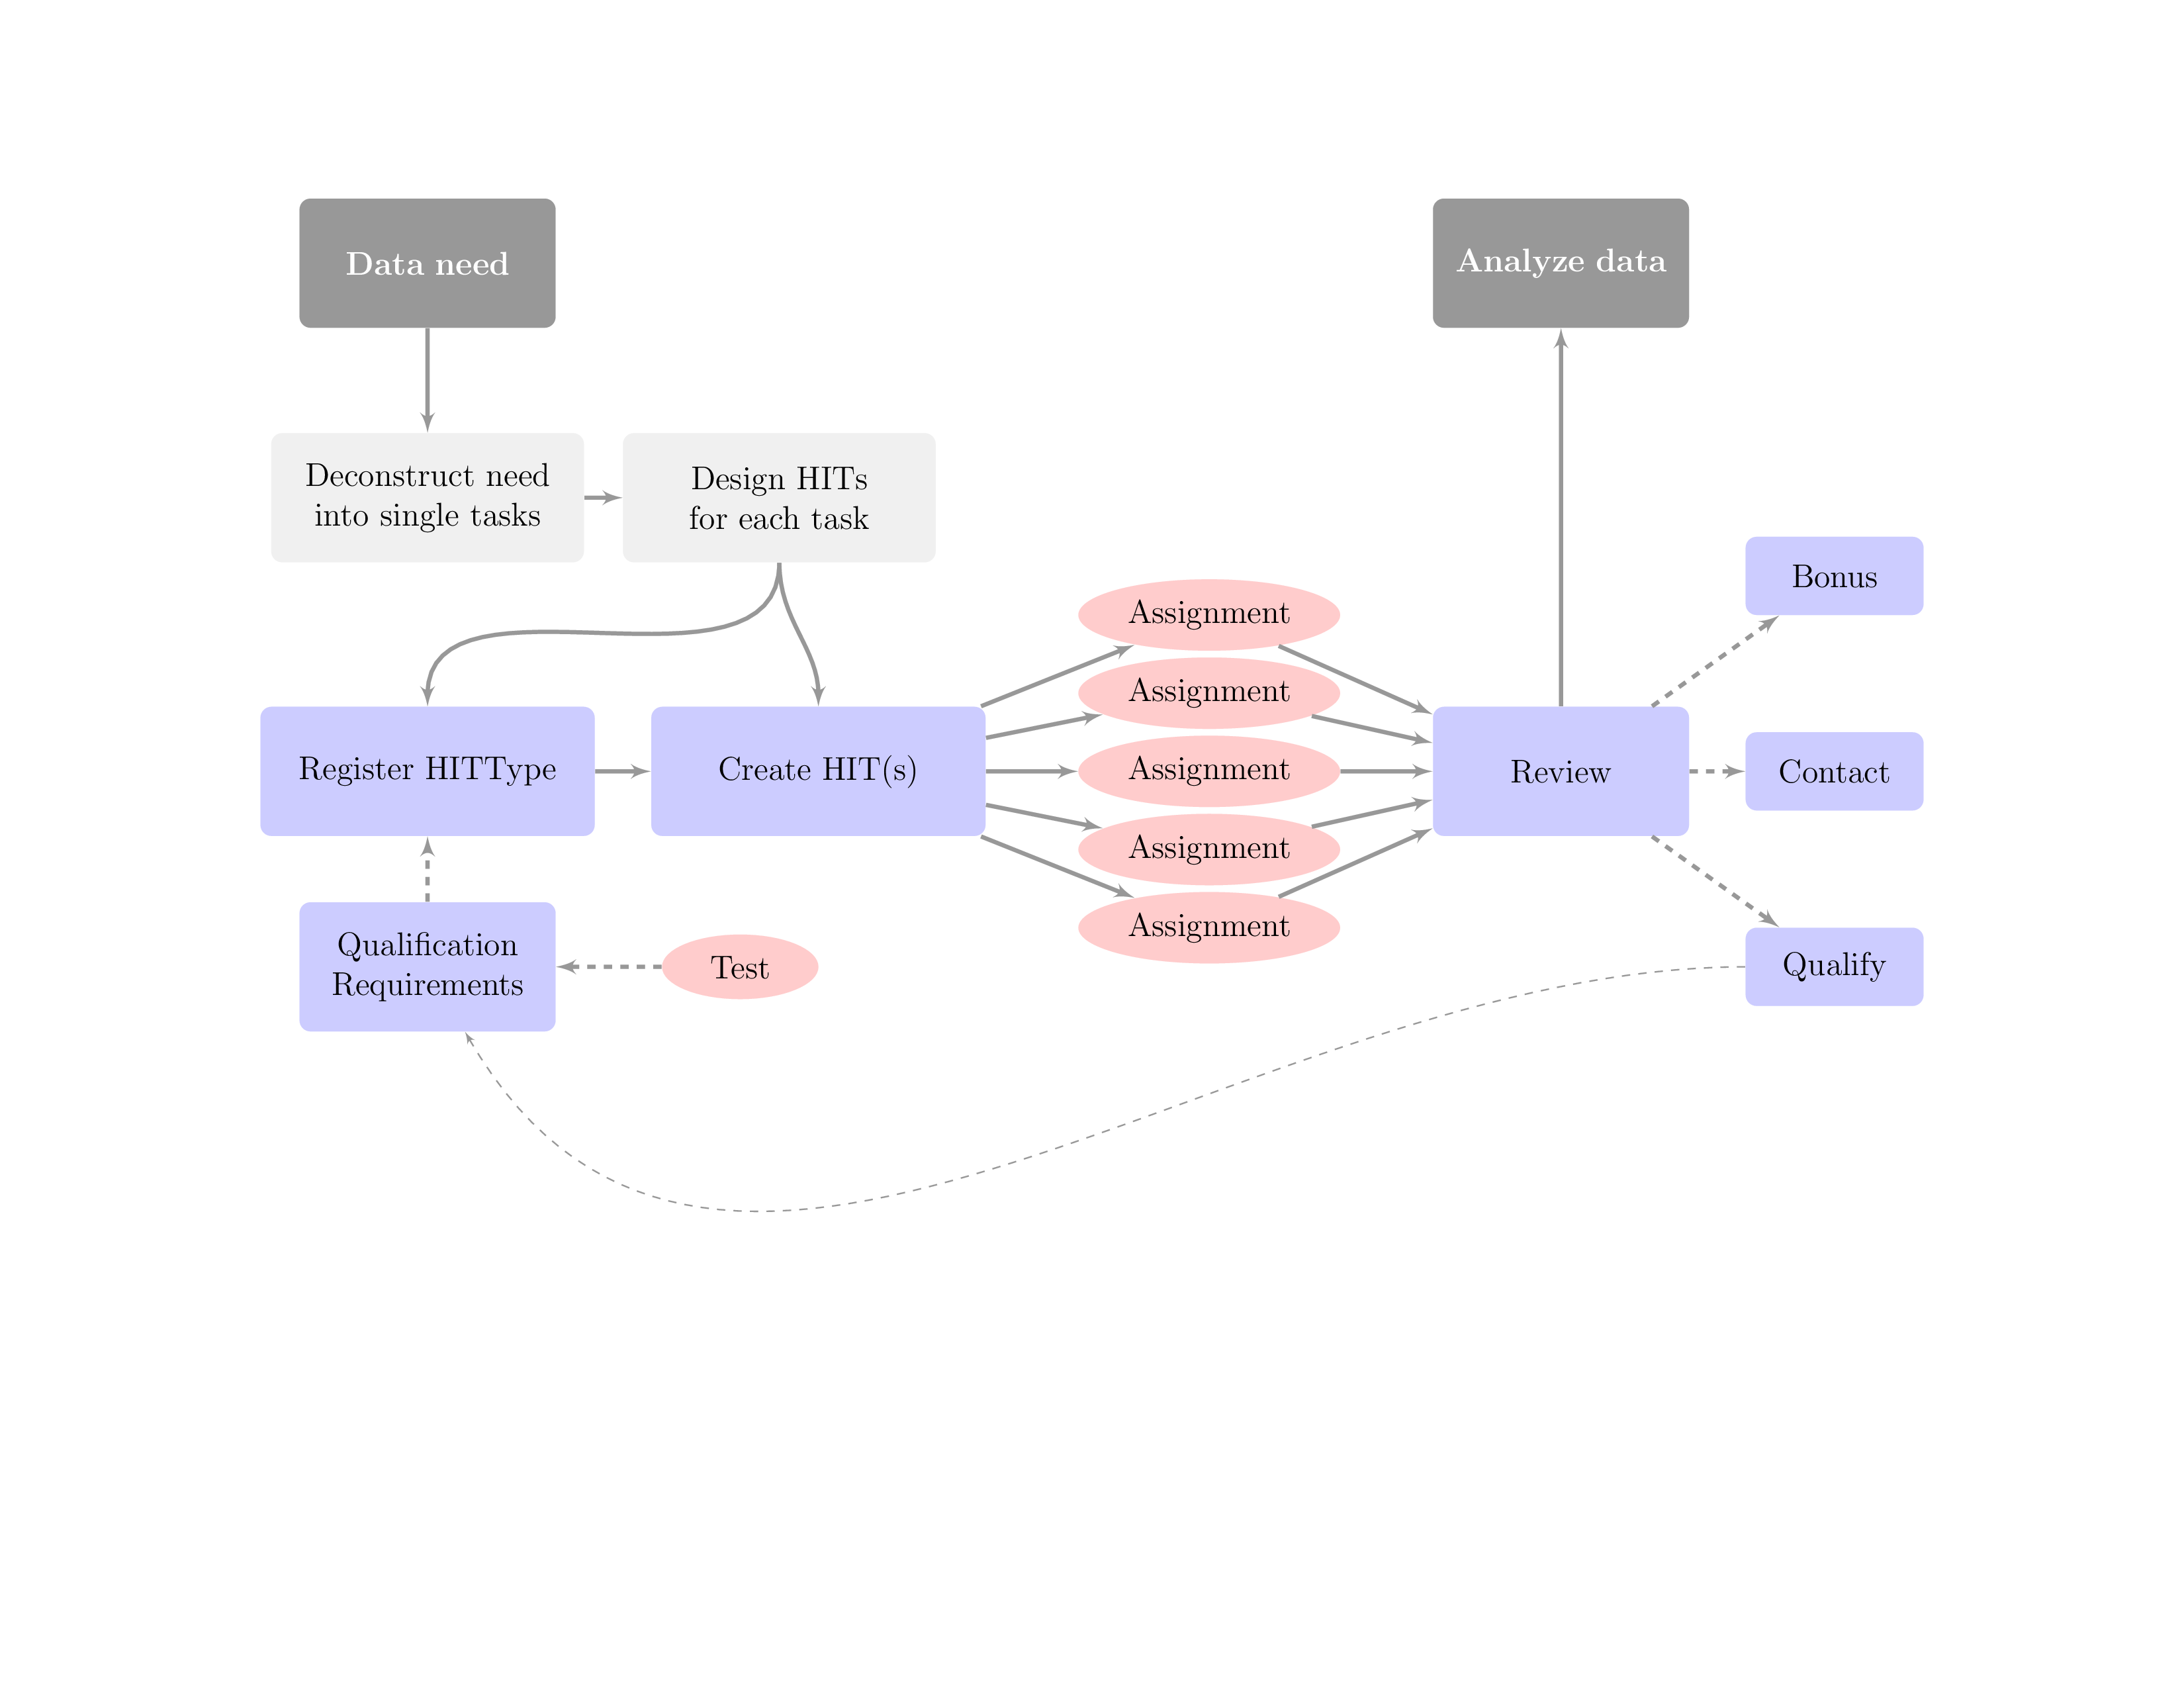
\includegraphics[trim=1in 2.25in 1in 1in, clip=true, width=.7\textwidth]{MTurkR-workflow}
\end{center}
\caption{An MTurk Workflow}\label{fig:workflow}
\end{figure*}

By providing direct and complete access to the API, MTurkR removes rather than imposes (as the RUI does) limitations on what researchers can crowdsource. To describe how researchers might utilize MTurk, this section provides two examples of MTurk as a social science data platform using MTurkR code to demonstrate how to easily manage that data collection. In both cases, a data need --- first, for human coding of newspaper articles and, second, participation in a panel experiment --- starts the research workflow and that need is broken down into MTurk HITs, which are completed by workers and reviewed by the requester via MTurkR, before the completed data are extracted from MTurk for analysis immediately in R. Figure \ref{fig:workflow} lays out this basic process with solid lines representing necessary actions and dashed lines showing optional actions.

\subsection{First Use Case: Content Analysis}

One of the most prevalent research techniques in political science is content analysis, be it coding of newspaper articles, images, speeches, campaign advertisements, or websites. While this is often done with an army of undergraduate research assistants or, more recently, via a number of automated techniques, crowdsourcing of human coding remains underutilized. Following the workflow described in Figure \ref{fig:workflow}, a coding task consists of a need for a rectangular, item-by-attribute dataset for all of the items to be coded (items for our purposes are newspaper articles). Deconstructing this need into individual tasks, requires the construction of a coding sheet to be used on each item (a HIT will consist of coding one item), which can be written as an HTML form (or prepared in WYSIWYG form in the RUI).

To ensure quality, however, it may also be useful to restrict who can code the items to those who have demonstrated that they can accurately perform the task. Thus, in addition to designing each of the HITs, a qualification test should also be designed that will simulate the coding process and allow the requester to evaluate whether or not a particular worker qualifies to work on the coding.\footnote{For technical reasons, this test needs to be written in the proprietary QuestionForm (XML) format, with the advantage being that MTurk can automatically score workers' qualification tests.} Once the coding sheet and qualification test are written, implementing the coding process via MTurkR simply proceeds left-to-right across the tasks in Figure \ref{fig:workflow}.

First, a HITType is created with the qualification test to display all of the coding items together on the MTurk worker site. Then, each HIT is created by associating it with the HITType. Workers then complete the qualification test and, if successful, are eligible to complete assignments. Once assignments are completed, the requester can review those assignments (approving acceptable work and rejecting all else) and then extract the data and analyze. Workers who pass the qualification test but fail to perform well on the work can have their qualification revoked, preventing them from completing more of the assignments. The HITType has four required and three optional characteristics, but good practice is to specify all of them:
\singlespacing\begin{itemize*}
\item Title (required)
\item Description (required)
\item Reward (required)
\item Duration (required)
\item Keywords
\item Assignment Auto-Approval Delay
\item Qualification Requirements
\end{itemize*}

\noindent To register a HITType, these characteristics need to be defined in a call to \verb|RegisterHITType()|. But, first, we will create a Qualification that tests workers' ability to code, along with an AnswerKey that MTurk will use to automatically score and qualify workers who complete the test.

% NEED TO SHOW A QuestionForm AND AnswerKey EXAMPLES, POSSIBLY IN APPENDIX?


\begin{Verbatim}[fontsize=\footnotesize, xleftmargin=3mm]
newqual <- CreateQualificationType(name="Coding Test", description="Test of coding ability",
                                   status="Active", test.duration=seconds(hours=1),
                                   test=QuestionForm, # a character string containing a QuestionForm
                                   answerkey=AnswerKey) # a character string containing an AnswerKey
\end{Verbatim}

\noindent That QualificationRequirement can then be attached to a new HITType, along with the other parameters:

\begin{Verbatim}[fontsize=\footnotesize, xleftmargin=3mm]
q1 <- GenerateQualificationRequirement(newqual$QualificationTypeId, ">=", 100, preview=TRUE)
register <- RegisterHITType(title="20-Question Survey",
                            description="Take a five-question survey about your political opinions 
                                         from researchers at Aarhus University.",
                            reward=".25", duration=seconds(days=1,hours=8),
                            keywords="survey, question, answers, research, politics",
                            qual.req=q1)
\end{Verbatim}

\begin{figure*}
\begin{center}
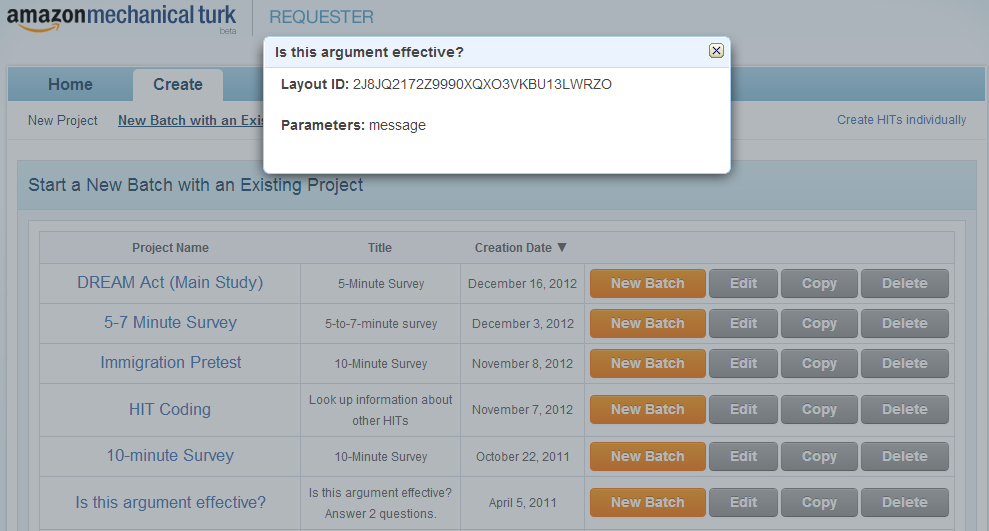
\includegraphics[width=.6\textwidth]{LayoutId2}
\end{center}
\caption{Retrieving a HIT LayoutId from the RUI}\label{fig:layout}
\end{figure*}

Creating a HIT using HITLayout parameters is also incredibly easy. The coding sheet template can be saved in the RUI with a placeholder of the style \verb|${message}| where the text of each article will be inserted. Once the HIT template is created in the RUI, you can retrieve its LayoutId from \url{https://requester.mturk.com/hit_templates} by clicking on the ``Project Name'' on the left-hand side of the screen. A pop-up window will appear displaying the LayoutId and the name of any placeholders (see Figure \ref{fig:layout}). Those placeholders can be replaced with the relevant material when \verb|CreateHIT()| is called, by specifying \verb|hitlayoutid| and \verb|hitlayoutparameters|. Assuming the newspaper texts are loaded into R in a list of character strings called \verb|articles|, one can simply iterate through that list to create each HIT, placing the text of each article in the \verb|message| layout parameter:

\begin{Verbatim}[fontsize=\footnotesize, xleftmargin=3mm]
layout <- "2J8JQ2172Z9990XQXO3VKBU13LWRZO"
hits <- vector(length=length(articles), mode="character")
for(i in 1:length(articles)){
   hits[i] <- CreateHIT(hit.type=register$HITTypeId, hitlayoutid=layout,
                        hitlayoutparameters=GenerateHITLayoutParameter("message",articles[[i]]),
                        annotation=paste("Article to code",i),
                        expiration=seconds(hours=1),
                        assignments=2)$HITId
}
\end{Verbatim}

\noindent This loop will return the HITId for each new HIT, which the above code stores in a character vector called \verb|hits|. The HITId for each HIT (and the \verb|annotation| value, which provides a private description of the HIT visible only to the requesters) can be retrieved at any time using \verb|SearchHITs()|. Once a HIT is created, the simplest (and perhaps modal) management strategy is to simply let it run its course, with workers completing some or all of the available assignments before the HIT expires. But, it is also helpful to be able to make certain changes to HITs after they have been created

To delay the expiration of HIT (e.g., because not all assignments have been completed), \verb|ExtendHIT(hit=hits$HITId[1], add.seconds=seconds(days=1))| extends the specified HIT(s) by the time specified in \verb|seconds()|. If intercoder reliability appears to be low, a call to\\ \verb|ExtendHIT(add.assignments=1)| increases the number of available assignments for all specified HITs by one (or more) to help resolve disagreement.\footnote{MTurk also provides ``review policy'' functionality to automatically respond to agreements or disagreements between workers' coding. See MTurk documentation.}

\begin{Verbatim}[fontsize=\footnotesize, xleftmargin=3mm]
ExtendHIT(hit.type=register, add.assignments=1)
\end{Verbatim}

\noindent To instead expire a HIT early (e.g., because there is an unanticipated problem with the HIT), simply call \verb|ExpireHIT()| with one or more HITIds specified. At the completion of data collection, the easiest method of reviewing workers' assignments is simply to retrieve all of the assignments and them approve them. \verb|ApproveAllAssignments()| can be specified with either a HITId or a HITTypeId. Once a HIT and all of its assignment data are no longer needed, \verb|DisposeHIT()| can optionally delete all data from the MTurk server.

\begin{Verbatim}[fontsize=\footnotesize, xleftmargin=3mm]
a <- hits$HITId[1]
b <- GetAssignments(hit=a, return.all=TRUE)
c <- ApproveAllAssignments(hit=a)
\end{Verbatim}

\subsection{Second Use Case: Panel Experiments}

The viability of MTurk as a platform for implementing social science experiments is well-understood, but the platform's comparative advantage for implementing complicated panel data collection is underappreciated, in part for technological reasons. The ability to recontact and pay large numbers of workers falls outside the functionality of the RUI. In this use case, the objective is to implement a three-wave panel experiment, where respondents are randomly assigned to a condition at $t1$, recontacted to participate in a follow-up wave with additional block-randomization at $t2$, and finally a second follow-up wave at $t3$. In contrast with the first use case, the first stages of the workflow here are relatively easy. First, an experimental survey instrument is constructed with any tool (e.g., Qualtrics or one's own HTML). Second, a single HIT is created (without a qualification test) to which workers respond by completing the survey-experiment. Note that when only one HIT is needed, the parameters normally assigned with \verb|RegisterHITType()| can be specified in the \verb|CreateHIT()| command.

\begin{Verbatim}[fontsize=\footnotesize, xleftmargin=3mm]
newhit <- CreateHIT(question=GenerateExternalQuestion("http://www.test.com/surveylink", 400)$string,
                    title="20-Question Survey",
                    description="Take a five-question survey about your political opinions.",
                    reward=".25",
                    duration=seconds(hours=4),
                    expiration=seconds(days=7),
                    assignments=1000,
                    keywords="survey, question, answers, research, politics, opinion",
                    auto.approval.delay=seconds(days=15),
                    qual.req=GenerateQualificationRequirement("Location","==","US",preview=TRUE))
\end{Verbatim}

\noindent Once a sufficient number of responses are collected (i.e., assignments completed) --- this can be checked with \verb|HITStatus(hit=newhit$HITId)|, assignments can be reviewed such that only those who pass an attention check are approved and the remainder rejected:
\begin{Verbatim}[fontsize=\footnotesize, xleftmargin=3mm]
review <- GetAssignments(hit=newhit$HITId)
correctcheck <- "7"
approve <- approve(assignments=review$AssignmentId[review$check==correct])
reject <- reject(assignments=review$AssignmentId[!review$check==correct])
\end{Verbatim}

After reviewing these assignments, MTurkR is leveraged via the three tasks at the right side of Figure \ref{fig:workflow}: Bonus, Contact, and Qualify. To implement a panel, workers who completed the original HIT (the $t1$ survey) are randomized to receive either a Democratic or Republican message in the $t2$ survey, with separate links for each condition. These workers are then contacted to complete the $t2$ survey and are paid a bonus if they complete it.

\begin{Verbatim}[fontsize=\footnotesize, xleftmargin=3mm]
random <- rbinom(dim(approve)[1], 1, .5)
b1 <- "If you complete a follow-up survey, you will receive a $.50 bonus.\n
       You can complete the survey at the following link: http://www.test.com/link1?WorkerId="
w1 <- approve$WorkerId[random==1]
t2cond1 <- ContactWorkers(subjects="Complete follow-up survey for $.50 bonus",
                          msgs=sapply(c1,FUN=function(worker) paste(b1,worker)), workers=w1)
b2 <- "If you complete a follow-up survey, you will receive a $.50 bonus.\n
       You can complete the survey at the following link: http://www.test.com/link2?WorkerId="
w2 <- approve$WorkerId[random==2]
t2cond2 <- ContactWorkers(subjects="Complete follow-up survey for $.50 bonus",
                          msgs=sapply(c2,FUN=function(worker) paste(b2,worker)), workers=w2)
\end{Verbatim}

The process could be repeated for the $t3$ survey. Paying bonuses for completing the $t2$ and $t3$ surveys is similar. The below example shows paying a single bonus, but replacing the single character strings with vectors of character strings allows multiple bonuses to be paid with one called to \verb|GrantBonus()|.

\begin{Verbatim}[fontsize=\footnotesize, xleftmargin=3mm]
bonus <- GrantBonus(workers="AZ3456EXAMPLE",
                    assignments="123RVWYBAZW00EXAMPLE456RVWYBAZW00EXAMPLE",
                    amounts="1.00", reasons="Thanks for completing the follow-up survey!")
\end{Verbatim}

\noindent Workers can optionally be granted qualifications, e.g., to allow those who respond to all panel waves to complete a future study or, alternatively, to prevent participants in this study from completing a similar study launched in the near future bringing the process back to the left side of Figure \ref{fig:workflow}. With all data collected, analysis can proceed.\footnote{If all three panel waves were created as HITs, qualifications would restrict the $t2$ and $t3$ surveys to workers who had completed $t1$ and the data could also be directly extracted from MTurk via MTurkR rather than having to be pooled from another survey tool.}

\section{APIs, Cloud Data, and Political Science}

As these two use cases have demonstrated, crowdsourcing (via MTurk) is a powerful addition to the political scientist's toolkit. By managing cloud-based data collection directly in R, this process is also relatively easy, done in a comfortable programming environment, and scientifically reproducible. But using MTurkR to connect with the MTurk API also shows that R can be an effective and easy-to-use way to work with cloud-based data. Currently, R has few packages that provide easy access to data APIs. One, \href{http://cran.r-project.org/web/packages/twitteR/}{twitteR} provides access to Twitter data. Alone it may not be immediately useful, but when used in combination with the U.S. federal government's \href{http://www.usa.gov/About/developer-resources/social-media-registry.shtml}{Social Media Registry API}, it should be relatively easy to track the Twitter activity of numerous government agencies. A second R package, \href{http://cran.r-project.org/web/packages/RWeather/RWeather.pdf}{RWeather} provides access to current weather from NOAA weather stations; a more useful package would tap the \href{http://www.wunderground.com}{wunderground.com} API, which is capable of providing robust, geocoded weather data going back decades. An enormous amount of data is also available from other APIs, such as those from \href{http://dev.bitly.com/}{Bitly} to track social sharing of links and \href{https://developers.google.com/youtube/analytics/}{YouTube Analytics API} to track liking, sharing, and commenting on YouTube videos, \href{http://data.worldbank.org/developers}{The World Bank}, \href{http://www.census.gov/developers/}{U.S. Census Bureau}, the \href{https://www.federalregister.gov/blog/learn/developers}{Federal Register}, \href{http://www.opencongress.org/about/code}{OpenCongress} and \href{http://www.govtrack.us/developers}{GovTrack}, several \href{http://developer.washingtonpost.com/applications}{Washington Post APIs} that track political contributions and White House visitors, and eventually the new \href{Congress.gov}{Congress.gov}, which aims to be a central repository for Congressional data available via APIs. Developing software that enables researchers to readily tap into these immense sources of data is an important task for political methodologists, who can develop tools that enable non-programmers to easily access these data.

\begin{comment}
\appendix

\section{Appendix: QuestionForm and AnswerKey for First Use Case}
\begin{Verbatim}[fontsize=\footnotesize]
QuestionForm <- '
<QuestionForm xmlns="http://mechanicalturk.amazonaws.com/AWSMechanicalTurkDataSchemas/
                     2005-10-01/QuestionForm.xsd">
  <Overview>
    <DisplayName>Instructions</DisplayName>
    <QuestionContent>
      <FormattedContent><![CDATA[
        <h1>Please read the following article and then answer the questions below.
            You must get every answer correct to pass the qualification test</h1>
		<h2>INSERT HEADLINE HERE</h2>
		<p>INSERT XHTML-FORMATTED ARTICLE TEXT HERE</p>
      ]]></FormattedContent>
    </QuestionContent>
  </Overview>
  <Question>
    <QuestionIdentifier>q1</QuestionIdentifier>
	<DisplayName>Question 1</DisplayName>
    <IsRequired>true</IsRequired>
	<QuestionContent>
      <FormattedContent><![CDATA[
        <p>TEXT OF FIRST QUESTION</p>
      ]]></FormattedContent>
	</QuestionContent>
    <AnswerSpecification>
      <SelectionAnswer>
        <StyleSuggestion>radiobutton</StyleSuggestion>
        <Selections>
          <Selection>
            <SelectionIdentifier>1</SelectionIdentifier>
            <Text>Response Option 1</Text>
          </Selection>
          <Selection>
            <SelectionIdentifier>2</SelectionIdentifier>
            <Text>Response Option 2</Text>
          </Selection>
          <Selection>
            <SelectionIdentifier>3</SelectionIdentifier>
            <Text>Response Option 3</Text>
          </Selection>
          <Selection>
            <SelectionIdentifier>4</SelectionIdentifier>
            <Text>Response Option 4</Text>
          </Selection>
        </Selections>
      </SelectionAnswer>
    </AnswerSpecification>
  </Question>
  <Question>
    <QuestionIdentifier>q2</QuestionIdentifier>
	<DisplayName>Question 2</DisplayName>
    <IsRequired>true</IsRequired>
    <QuestionContent>
      <FormattedContent><![CDATA[
        <p>TEXT OF SECOND QUESTION</p>
      ]]></FormattedContent>
	</QuestionContent>
    <AnswerSpecification>
      <SelectionAnswer>
        <StyleSuggestion>radiobutton</StyleSuggestion>
        <Selections>
          <Selection>
            <SelectionIdentifier>1</SelectionIdentifier>
            <Text>Response Option 1</Text>
          </Selection>
          <Selection>
            <SelectionIdentifier>2</SelectionIdentifier>
            <Text>Response Option 2</Text>
          </Selection>
          <Selection>
            <SelectionIdentifier>3</SelectionIdentifier>
            <Text>Response Option 3</Text>
          </Selection>
          <Selection>
            <SelectionIdentifier>4</SelectionIdentifier>
            <Text>Response Option 4</Text>
          </Selection>
        </Selections>
      </SelectionAnswer>
    </AnswerSpecification>
  </Question>
</QuestionForm>'

AnswerKey <- '
<AnswerKey xmlns="http://mechanicalturk.amazonaws.com/AWSMechanicalTurkDataSchemas/
                  2005-10-01/AnswerKey.xsd">
  <Question>
    <QuestionIdentifier>q1</QuestionIdentifier>
    <AnswerOption>
      <SelectionIdentifier>3</SelectionIdentifier>
      <AnswerScore>50</AnswerScore>
    </AnswerOption>
  </Question>
  <Question>
    <QuestionIdentifier>q2</QuestionIdentifier>
    <AnswerOption>
      <SelectionIdentifier>1</SelectionIdentifier>
      <AnswerScore>50</AnswerScore>
    </AnswerOption>
  </Question>
</AnswerKey>'
\end{Verbatim}
\end{comment}

%%%%%%%%%%%%%%%%%%%%%%%%%%%%%%%%%%%%%%%%%%%%%%%%
\singlespacing
\bibliographystyle{apsa-leeper}
\bibliography{MTurkR}
%%%%%%%%%%%%%%%%%%%%%%%%%%%%%%%%%%%%%%%%%%%%%%%%

\end{document}